\beginsong{Als in de mei}
\beginverse
Als in de mei, de blijde mei,
de merel fluit in 't woud,
ja fluit in 't woud,
dan trekken jonge kerels, 
van niets benauwd,
dan trekken jonge kerels, 
van niets benauwd.
\endverse
\beginchorus
Juvi valle valle valle valle lala
Juvi valle valle valle valle lala
Dan trekken jonge kerels, 
van niets benauwd.
\endchorus
\beginverse
Zij zingen luid hun lustig lied,
dat 't galme door het woud, 
ja door het woud.
Ze stappen 't leven tegen, 
van niets benauwd,
ze stappen 't leven tegen, 
van niets benauwd.
\endverse
\beginverse
Ach fiere jeugd, ach fiere jeugd,
uw lied klinkt veel te stout, 
ja veel te stout.
Ge zult wel anders zingen,
wordt gij eens oud,
Ge zult wel anders zingen,
wordt gij eens oud.
\endverse
\beginverse
Wij zingen nooit een ander lied,
al klinkt het nog zo stout,
ja nog zo stout.
Wij stoere vlaamse kerels, 
nooit worden w' oud,
wij stoere vlaamse kerels, 
nooit worden w' oud.
\endverse
\endsong
\begin{intersong}
    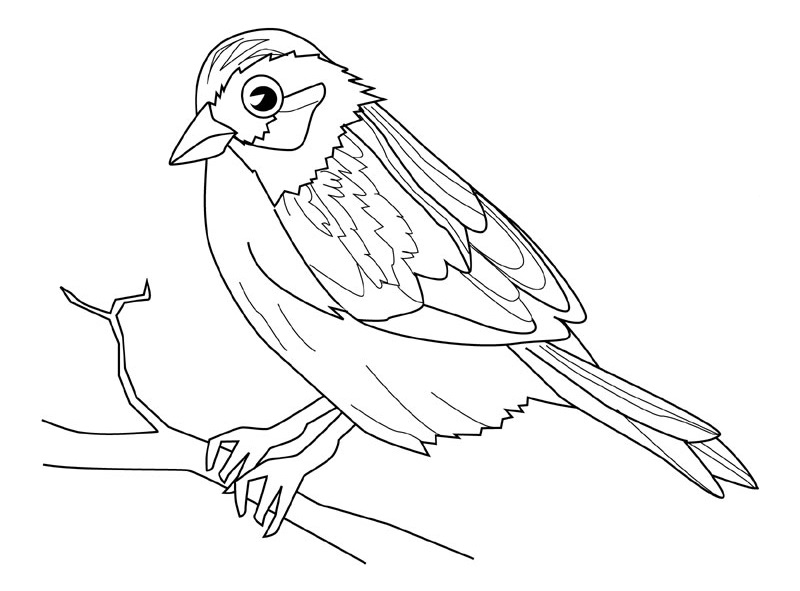
\includegraphics[width=0.4\textwidth]{img4}
\end{intersong}